	\newpage
\section{Projektowanie}		%3
%Opis przygotowania narzędzi (git, visual studio). Wybór i opis bibliotek, klas. Szkic layoutów. Pseudo kody. Opisy wykorzystanych algorytmów (np. algorytm sortowania). Dokładniejsze określenie założeń i działania aplikacji, (np.: ten przycisk otworzy takie okno a w tym oknie wpisujemy takie dane).

\subsection{Przygotowanie narzędzi (Git, Visual Studio)}		%3.1

\subsubsection{Visual Studio} %3.1.1
\hspace{0.60cm}Pierwszym i oczywistym krokiem, który musimy wykonać jest przygotowanie właściwych technologii i środowisk, które posłużą do tworzenia naszego projektu. Jako środowisko programistyczne wybrano Visual Studio 2022 i dostępną na nim wspomnianą wcześniej platformę Xamarin.Forms. W celu instalacji tego narzędzia, pobieramy plik instalacyjny odpowiedni dla naszego systemu ze strony Microsoftu\footnote{Plik instalacyjny na stronie  https://visualstudio.microsoft.com/pl/vs\cite{www1}.}, co pokazano na rysunku \ref{rys:rysunek002a}. Podczas instalacji, w menedżerze pakietów, wybieramy pakiety \textit{Mobile i desktop developement with ASP.NET}, (rys. \ref{rys:rysunek002b}), zaznaczając też opcjonalne dodatki w zależności od wymagań (rys. \ref{rys:rysunek002c})(np. Xamarin, emulator Androida itd.). Środowisko Visual Studio posiada zintegrowany system kontroli wersji oprogramowania Git, który będzie wspomagał naszą pracę.

\begin{figure}[!htb]
	\centering
	
\includegraphics[width=0.8\linewidth]{rys/vs1.png}
	\caption{Pobranie pliku instalacyjnego}
	\label{rys:rysunek002a}
\end{figure}

\begin{figure}[!htb]
	\centering
	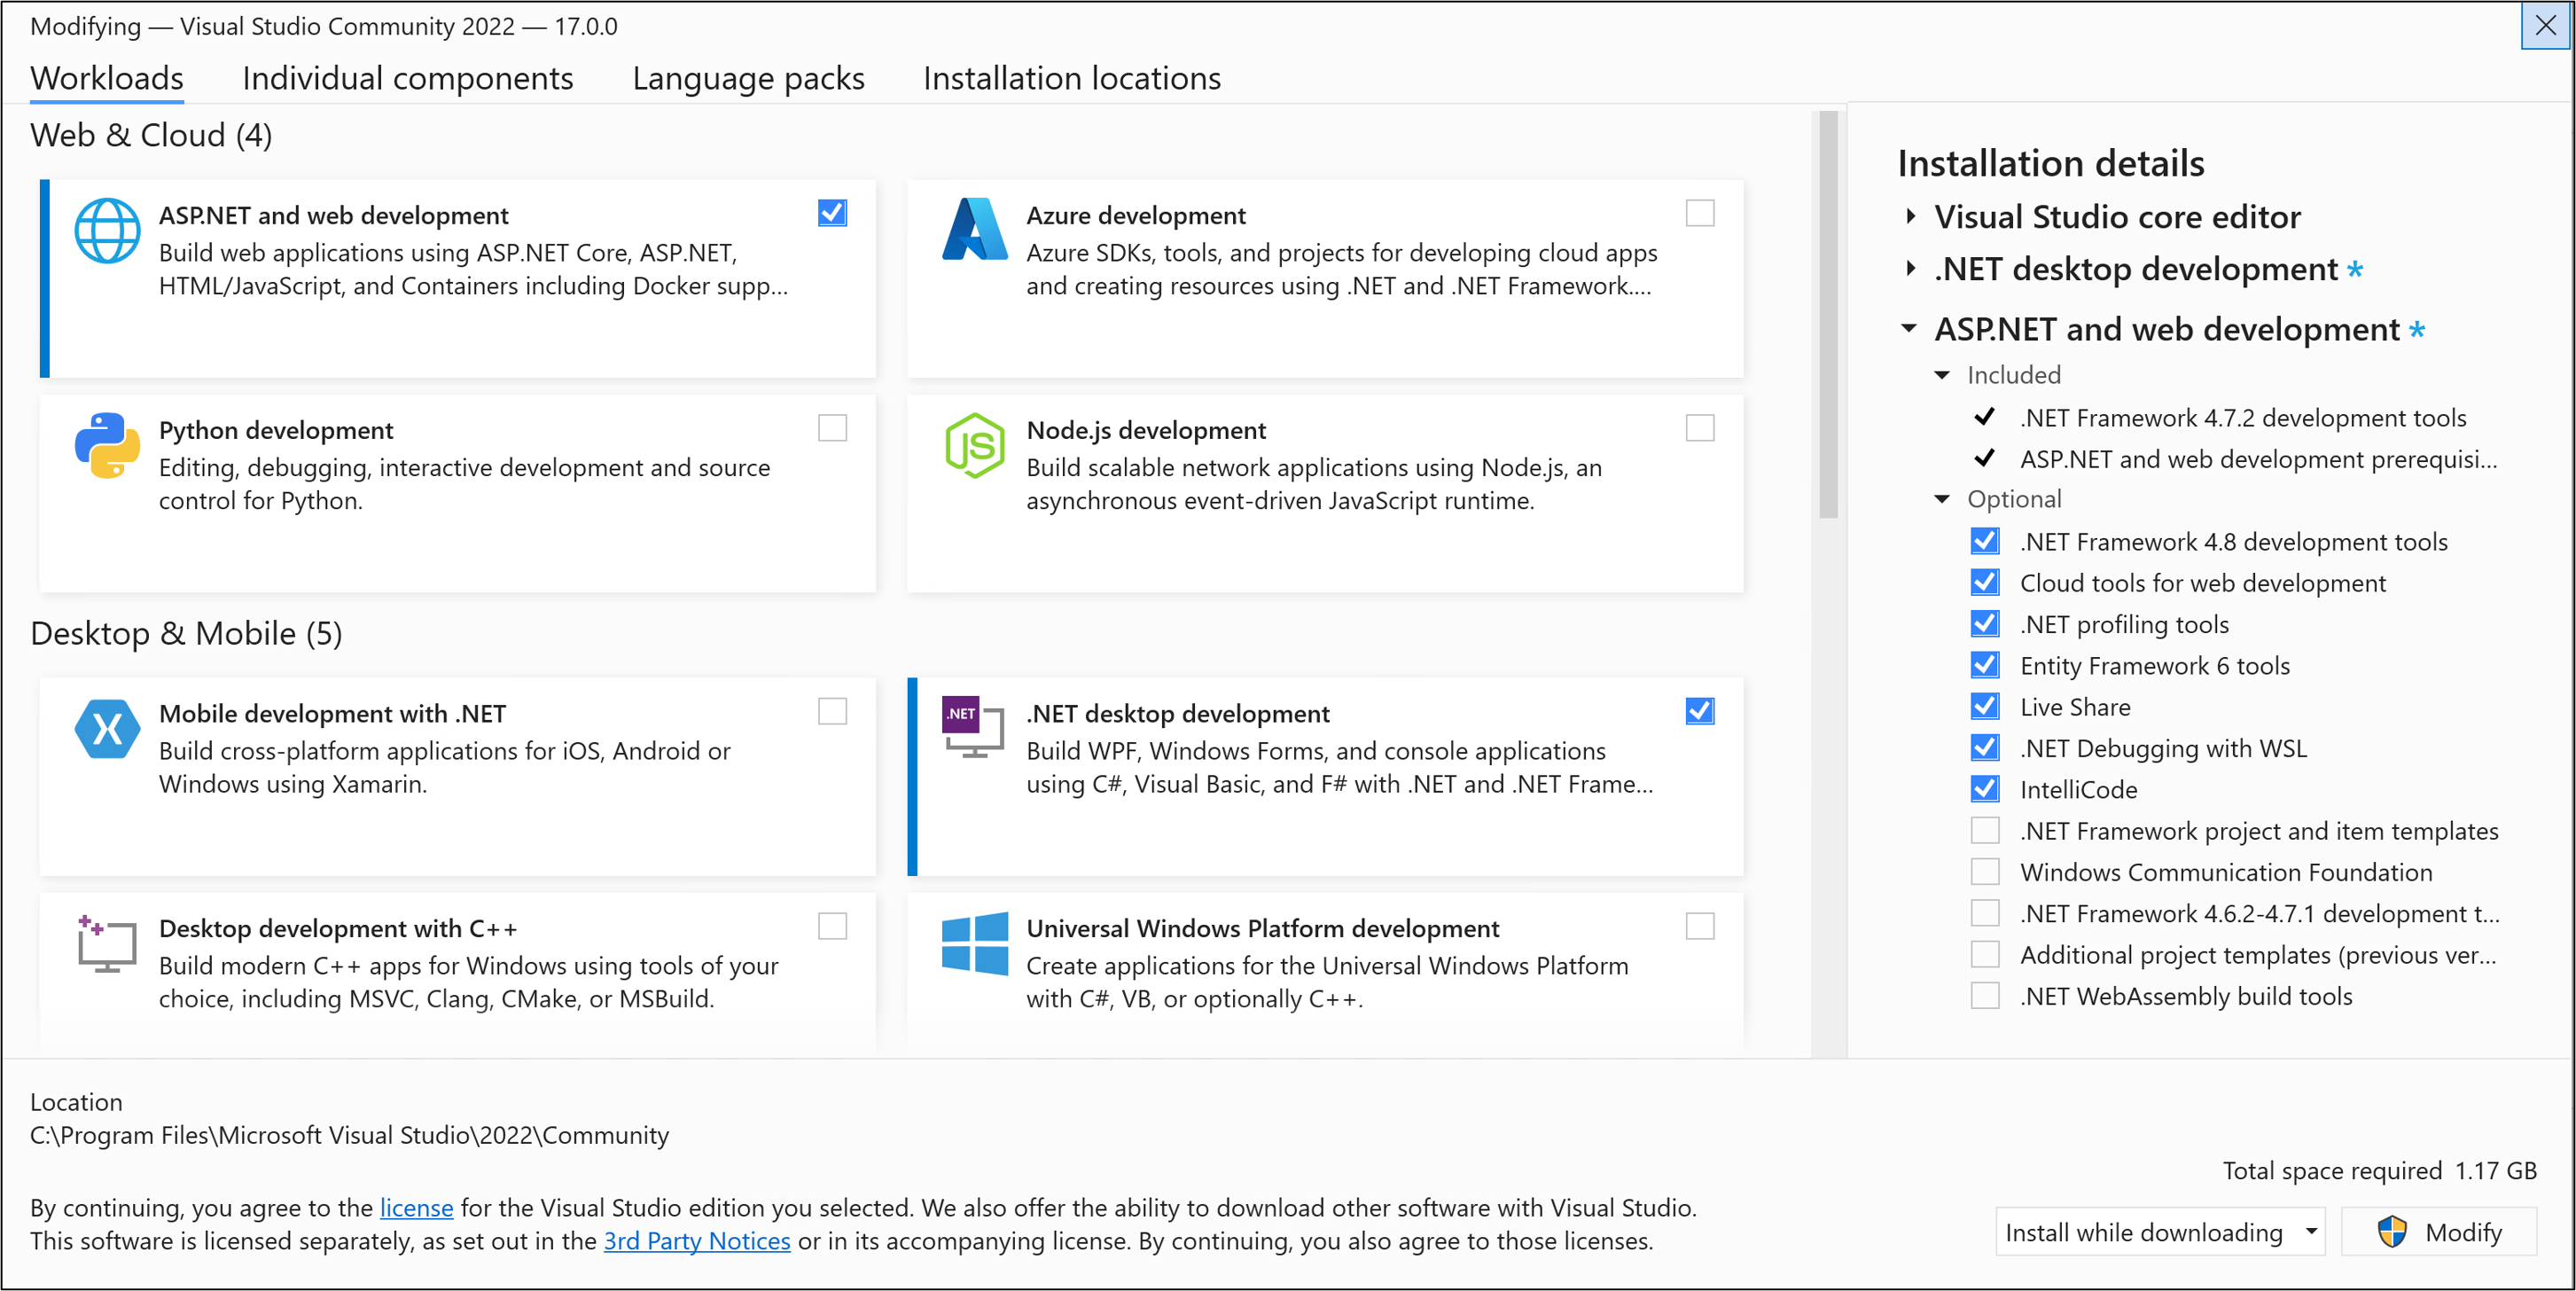
\includegraphics[width=0.8\linewidth]{rys/vs2.png}
	\caption{Wybór pakietów}
	\label{rys:rysunek002b}
\end{figure}

\begin{figure}[!htb]
	\centering
	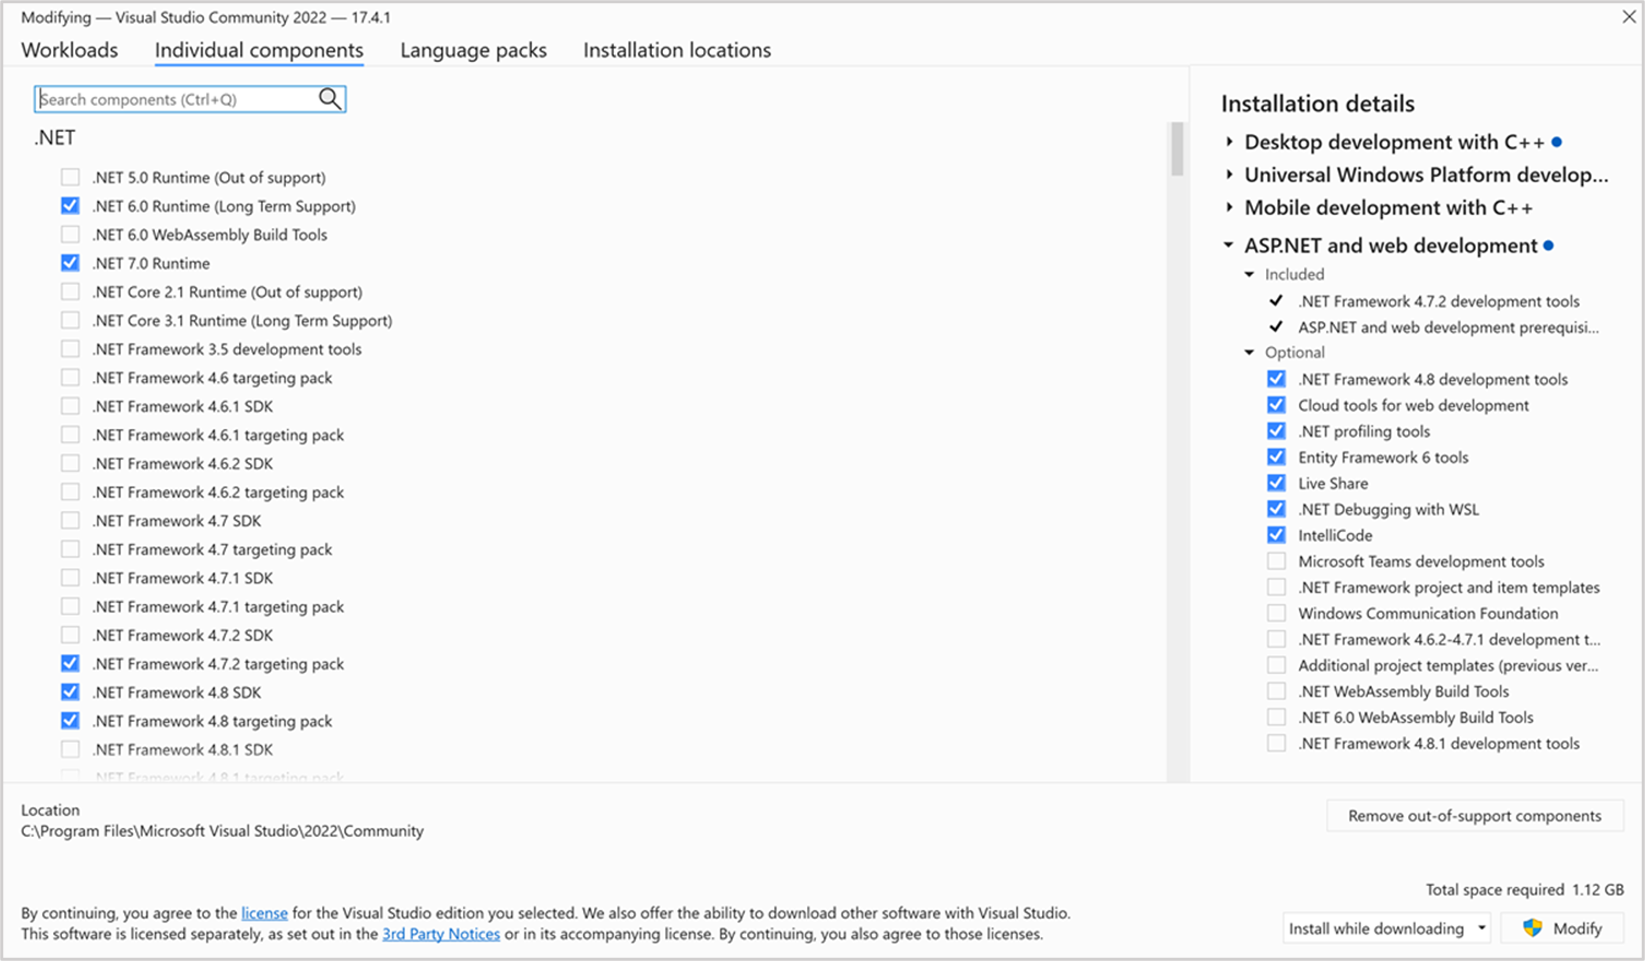
\includegraphics[width=0.8\linewidth]{rys/vs3.png}
	\caption{Dodatkowe pakiety i narzędzia}
	\label{rys:rysunek002c}
\end{figure}

\subsubsection{Git} %3.1.2

\hspace{0.60cm}Na stronie Github stworzone zostało zdalne repozytorium, do którego wysyłane będą kolejne wersje naszego projektu, z możliwością kontrybucji ze strony członków zespołu programistów. Lokalnie, na maszynach programistów zainstalowano dodatkowe narzędzie jakim jest desktopowa aplikacja Git for Windows, która dostarcza emulację BASH wykorzystywaną do uruchamiania Git'a z wiersza poleceń. Jest to duże udogodnienie dla osób, które czują się pewniej pracując z terminalem systemu Linux. Plik instalacyjny można pobrać ze strony\footnote{Plik instalacyjny na stronie https://git-scm.com/download/win\cite{www2}.}.

\subsection{Szkice layoutów}		%3.2

\subsubsection{Zakładka Kroki} %3.2.1

\hspace{0.60cm}W zakładce Kroki rys. \ref{rys:rysunek001a} (s. \pageref{rys:rysunek001a}) wyświetalana zostaje aktualna, obliczana w czasie rzeczywistym liczba odbytych kroków od czasu rozpoczęcia treningu. Początkowo liczba kroków równa się 0. Aplikacja liczy kroki od momentu nasiśnięcia przycisku \textbf{Start} w zakładce Trening (s. \pageref{rys:rysunek001b}). Liczenie kroków dokonuje się z wykorzystaniem modułu akcelerometra. Akcelerometr to wbudowany komponent do pomiaru przyspieszenia dowolnego urządzenia mobilnego. Ruchy takie jak kołysanie, przechylanie, obracanie, drżenie są wykrywane za pomocą akcelerometru. Wartość XYZ służy do obliczania i wykrywania ruchów. Współrzędne X, Y oraz Z reprezentują kierunek i położenie urządzenia wg. tych osi, w którym nastąpiło przyspieszenie. Dodatkowo przyspieszenie urządzenia obejmuje również przyspieszenie ziemskie (g = 9,81m/s2), które również należy uwzględnić w celu dokłądnego pomiaru.

Obliczanie ogólnego przyspieszenia urządzenia polega na pobieraniu z sensora wartości odpowiednio X, Y oraz Z. Następnie wartości te podstawiane są do odpowiedniego wzoru $\sqrt{(X*X + Y*Y + Z*Z) - 9,81}$, który wykorzystuje też wartość przyspieszenia ziemskiego. Zliczanie kolejnych kroków, począwszy od wartości 0, wykonuje się przy pomocy instrukcji warunkowej if oraz pętli for. Dodatkowo, celu niwelacji niedokładności w pomiarach, zliczane są one dopiero po odbyciu 6 kroków. Listing \ref{lst:listing-ps1} przedstawia za pomocą pseudokodu ogólną zasadę obliczania przyspieszenia:

\begin{lstlisting}[caption=Pseudokod działania krokomierza, label={lst:listing-ps1}, language=C++]
	Lista Zawierajaca_Wartosci_Przyspieszen;
	zmienna X = Odczyt.Sensora.X;
	zmienna Y = Odczyt.Sensora.Y;
	zmienna Z = Odczyt.Sensora.Z;
	
	zmienna Przyspieszenie = \sqrt{(X*X + Y*Y + Z*Z) - 9,81};
	
	JESLI (liczba_Wartosci_Przyspieszen > 1)
	{
		pomiar_krokow = 0;
		DLA (i = 1; i < liczba_Wartosci_Przyspieszen - 1; i++)
		{
			pomiar_krokow++;
			JESLI (liczba_krokow > 5)
			{
				liczba_krokow += 6;
			}
		}
	}
\end{lstlisting}

\begin{figure}[!htb]
	\centering
	
\includegraphics[width=.2\linewidth]{rys/kroki2.jpg}
	\caption{Layout krokomierza}
	\label{rys:rysunek001a}
\end{figure}

\subsubsection{Zakładka Trening} %3.2.2

\hspace{0.60cm}W zakładce Trening rys. \ref{rys:rysunek001b} (s. \pageref{rys:rysunek001b}) użytkownik ma możliwość rozpoczęcia treningu. Naciśnięcie przycisku \textbf{Start} Zaczyna się odliczanie i wyświetlanie na ekranie bieżącego czasu odbywanego treningu, pokonany dystans w metrach, bieżąca prędkość oraz teoretyczna ilość spalonych kalorii. Na środkowej części ekranu wyświetlana zostaje, przy wykorzystaniu modułów GPS oraz  Map Google bieżąca lokalizacja użytkownika. Za pomocą polilinii rysowana jest trasa, którą udaje się użytkownik. 

\begin{figure}[!htb]
	\centering
	\begin{minipage}{.5\textwidth}
		\centering
		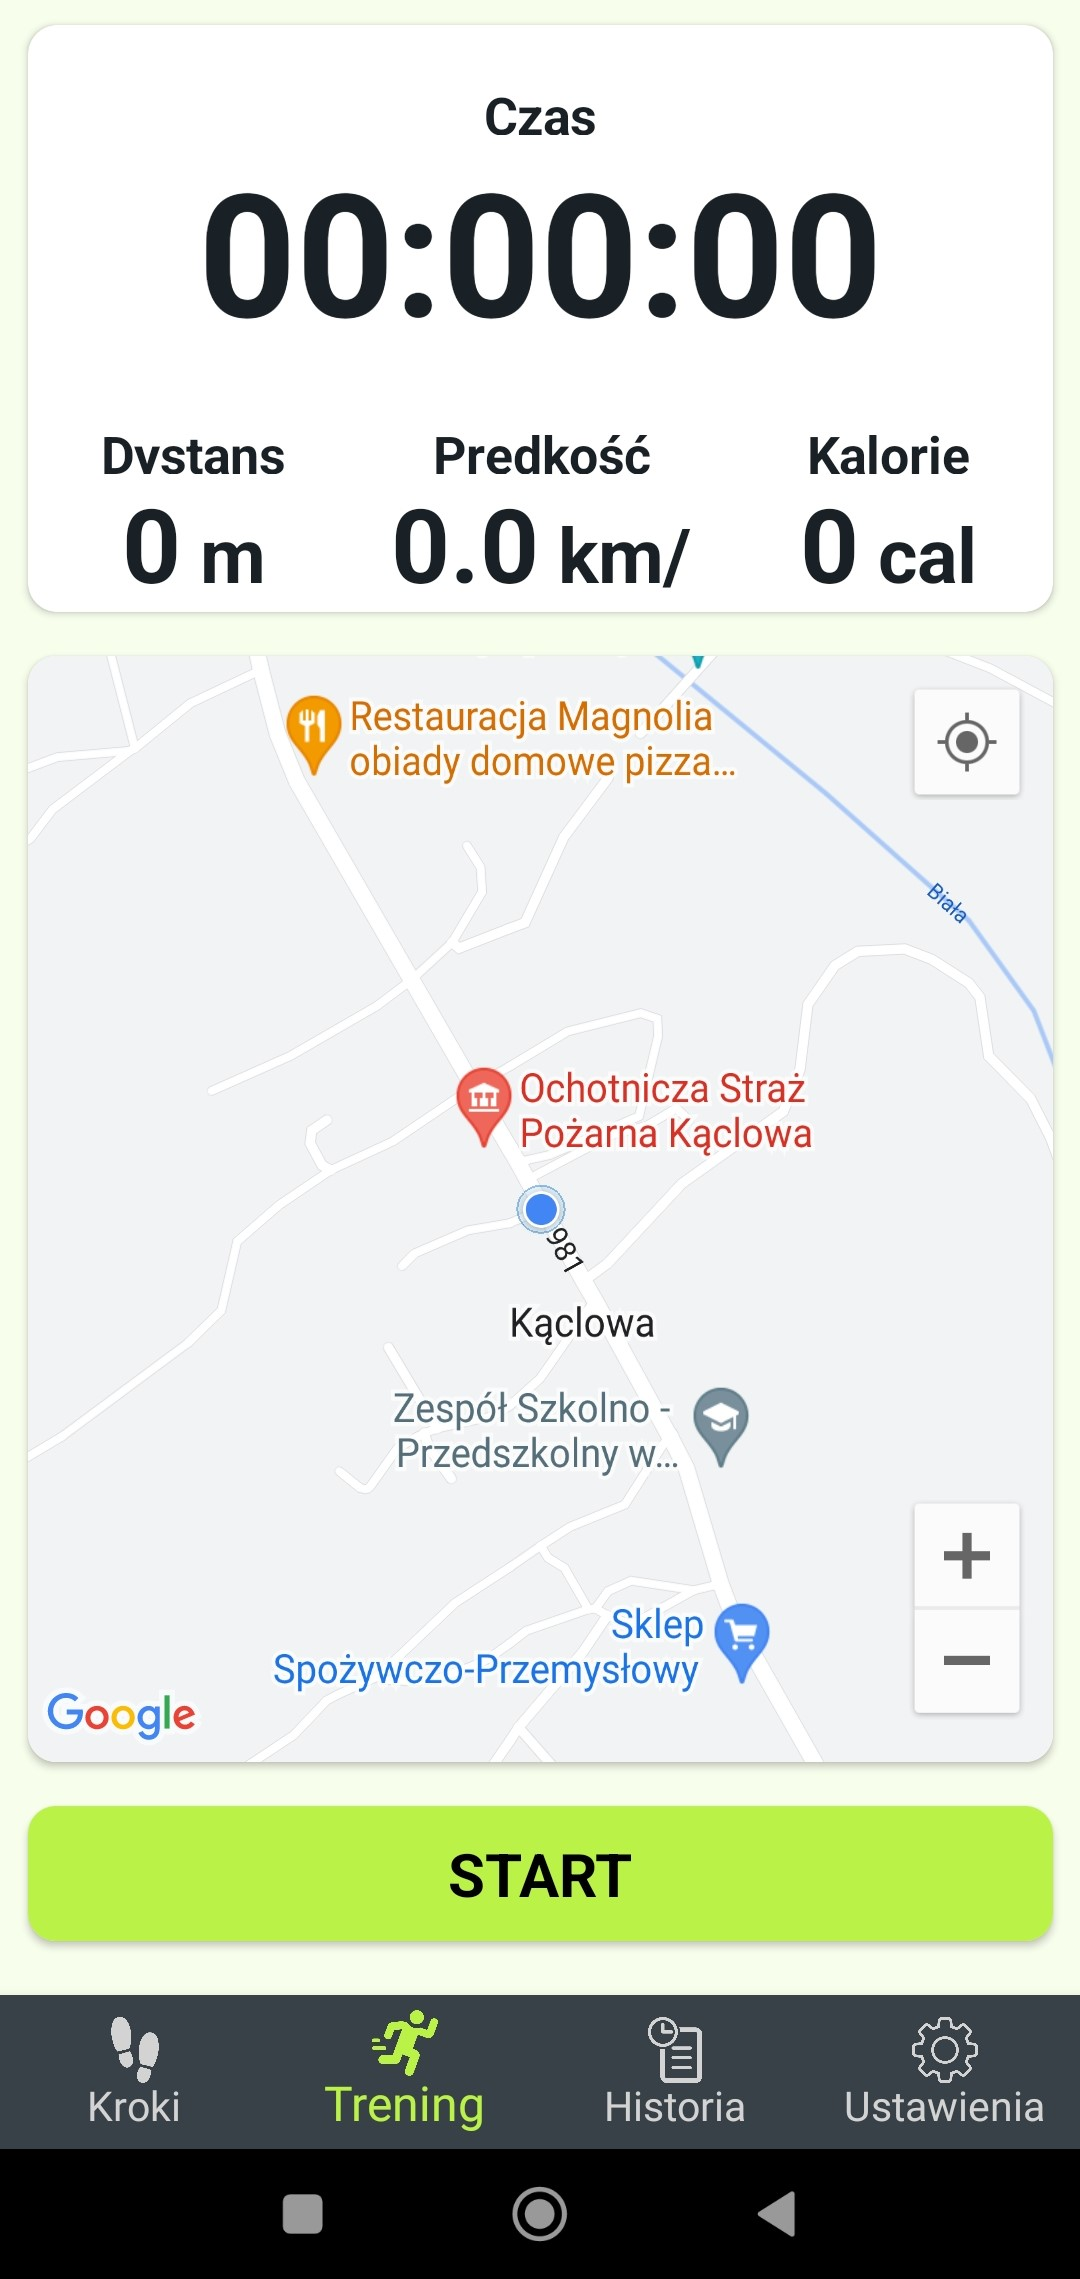
\includegraphics[width=.4\linewidth]{rys/trening1.jpg}
		\caption{Layout treningu - rozpoczęcie treningu}
		\label{rys:rysunek001b}
	\end{minipage}%
	\begin{minipage}{.5\textwidth}
		\centering
		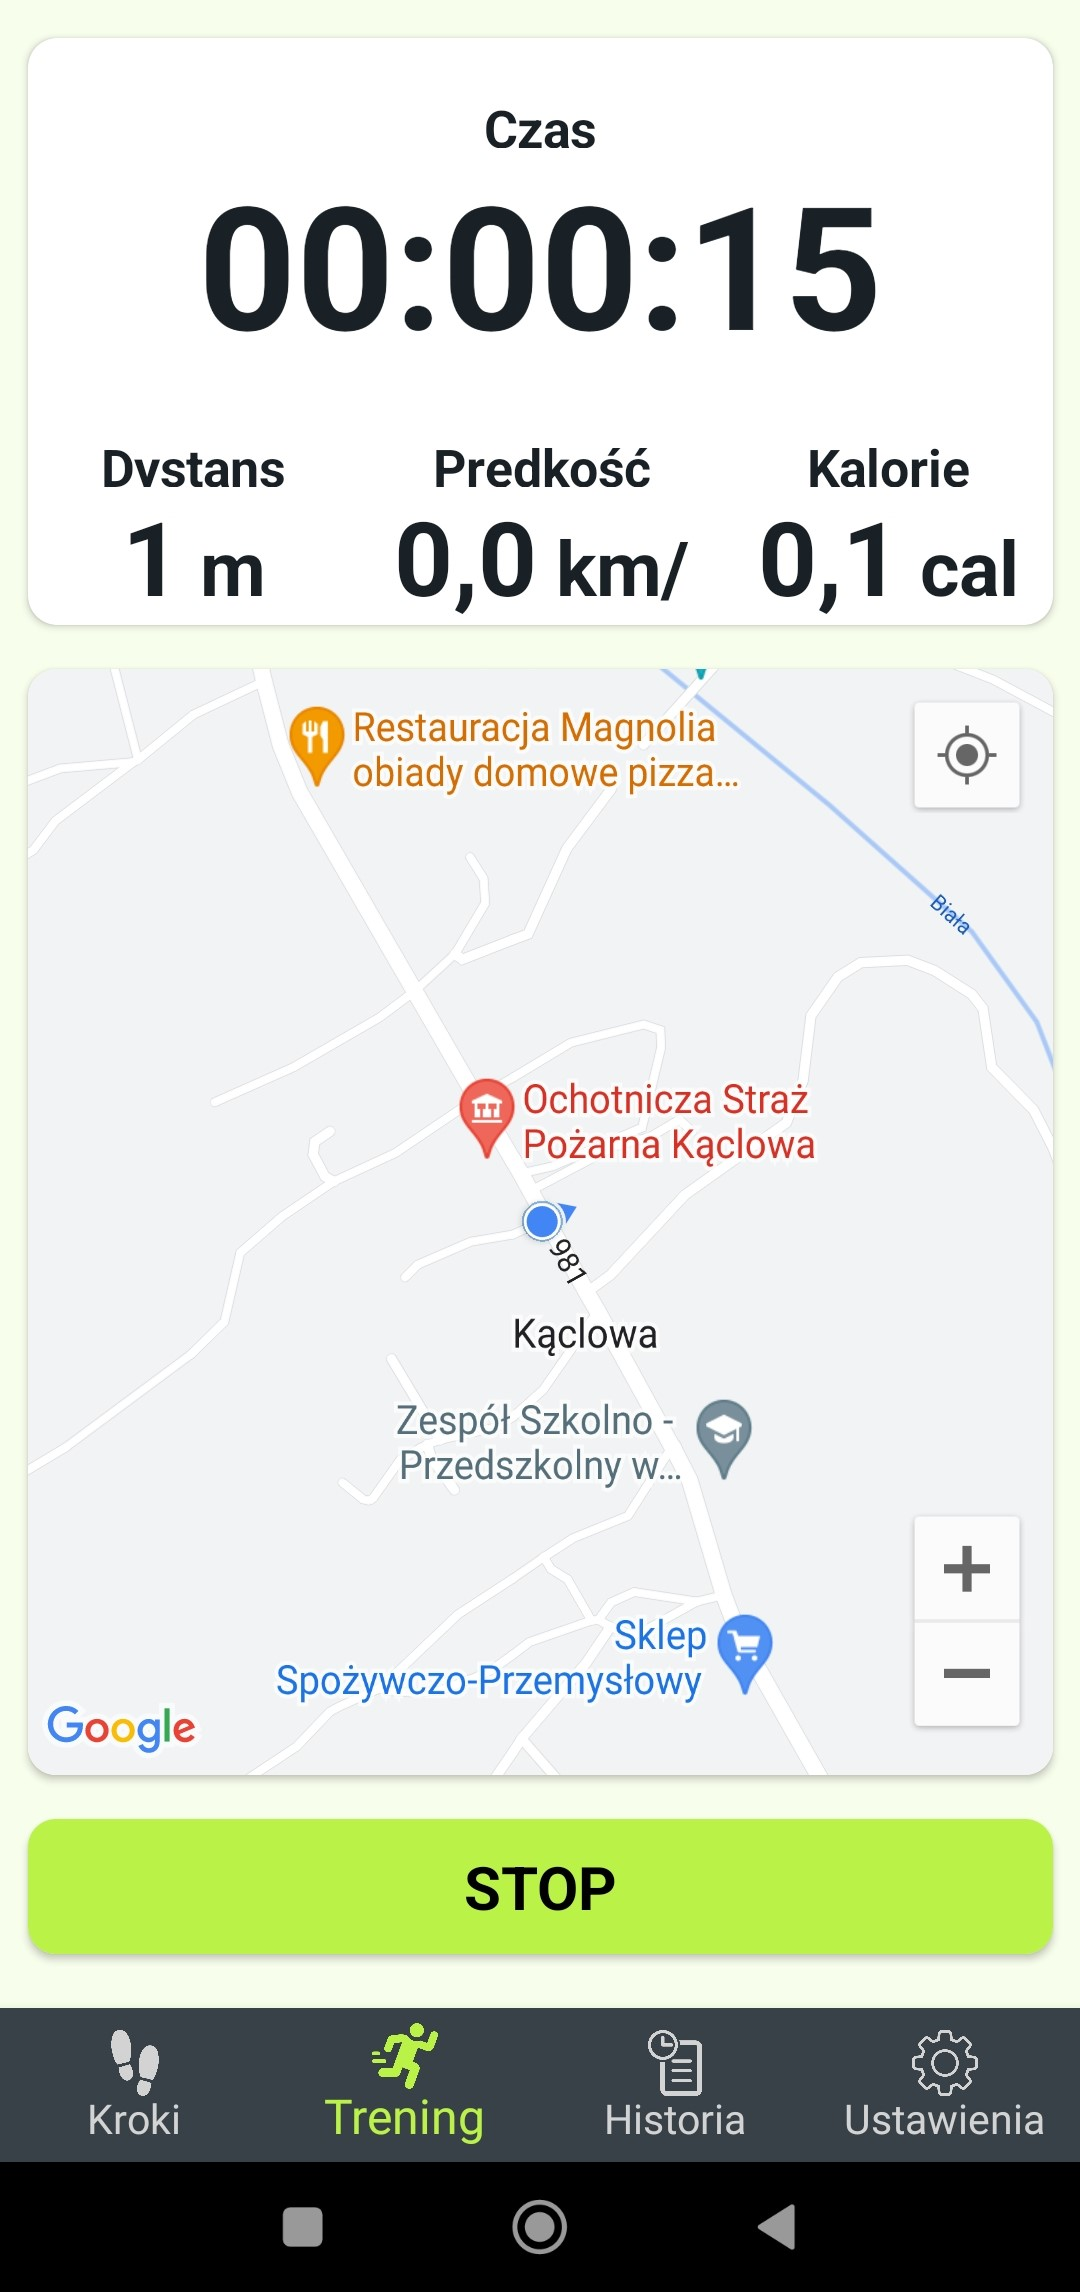
\includegraphics[width=.4\linewidth]{rys/trening1a.jpg}
		\caption{Zatrzymanie treningu}
		\label{rys:rysunek001ba}
	\end{minipage}
\end{figure}

\begin{figure}[!htb]
	\centering
	\begin{minipage}{.5\textwidth}
		\centering
		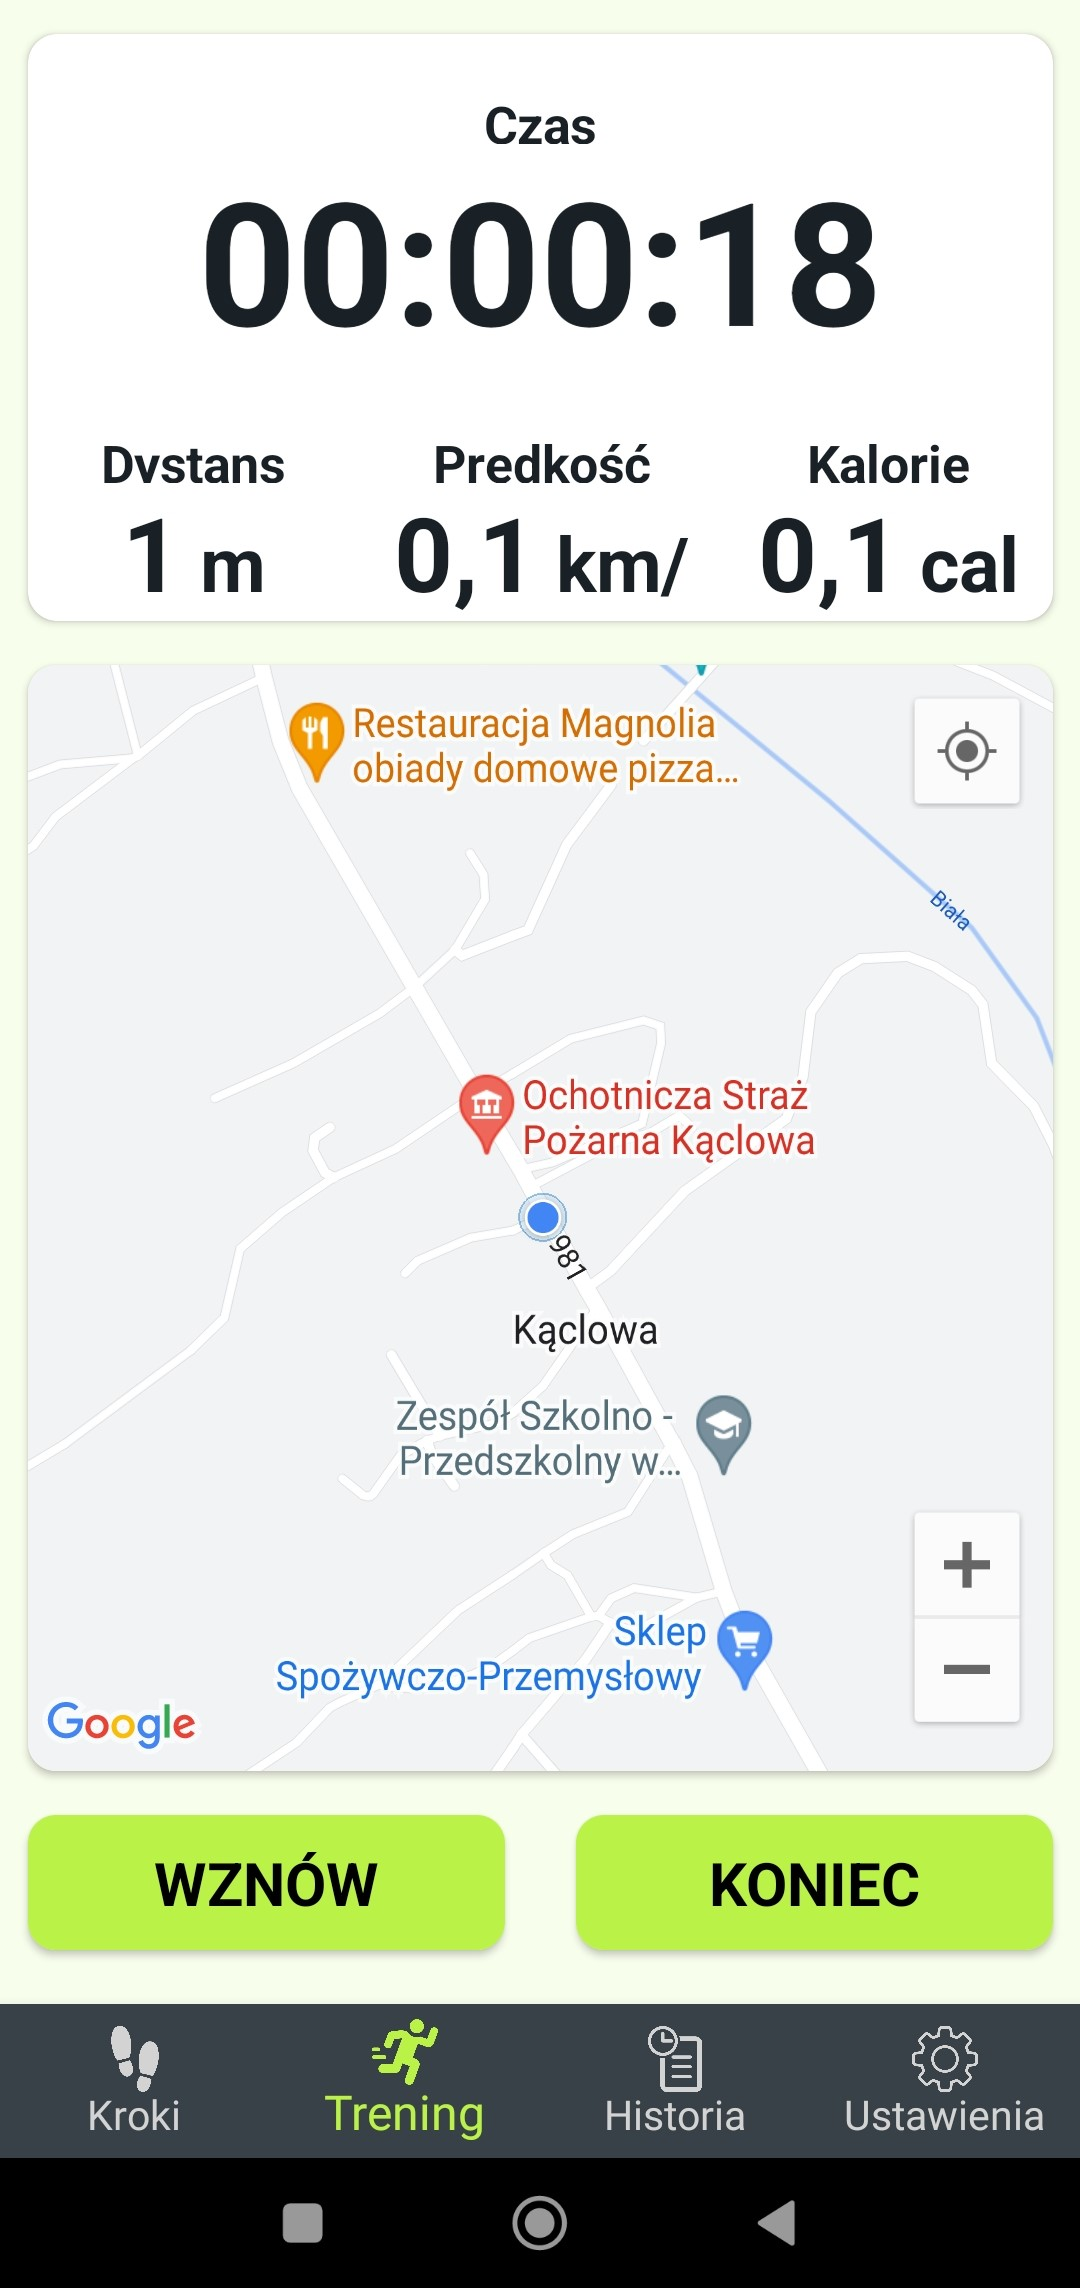
\includegraphics[width=.4\linewidth]{rys/trening1b.jpg}
		\caption{Wznowienie lub zakończenie treningu}
		\label{rys:rysunek001bb}
	\end{minipage}%
	\begin{minipage}{.5\textwidth}
		\centering
		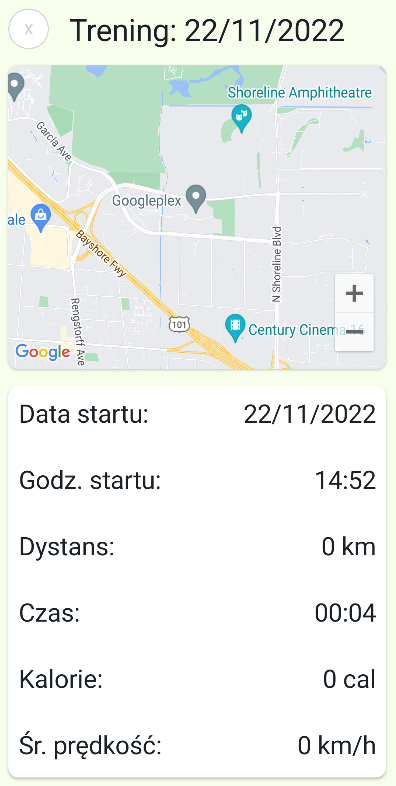
\includegraphics[width=.4\linewidth]{rys/trening2.png}
		\caption{Ekran podsumowania}
		\label{rys:rysunek001c}
	\end{minipage}
\end{figure}

Po zakończeniu treningu, w tej samej zakładce, wyświetlony zostaje ekran zawierający podsumowanie odbytego treningu. Jak pokazano na rys. \ref{rys:rysunek001c} (s. \pageref{rys:rysunek001c}), podsumowanie zawiera datę i czas rozpoczęcia treningu, przebyty dystans, czas treningu, spalone kalorie oraz średnią prędkość z jaką poruszał się użytkownik. 

\subsubsection{Zakładka Historia} %3.2.3

\hspace{0.60cm}W zakładce Historia, po zakończeniu kolejnych treningów, do bazy danych zapisywane są rekordy zawierające dane dotyczące odbytych w przeszłości treningów wraz z podstawywymi danymi jak data, czas oraz statystyki, co pokazano na rys. \ref{rys:rysunek001d} (s. \pageref{rys:rysunek001d}). Dane po zakończeniu treningu są najpierw zapisywane do bazy danych SQLite, następnie wyświetlane w zakładce Historia od najnowszego do najstarszego.

\begin{figure}[!htb]
	\centering
	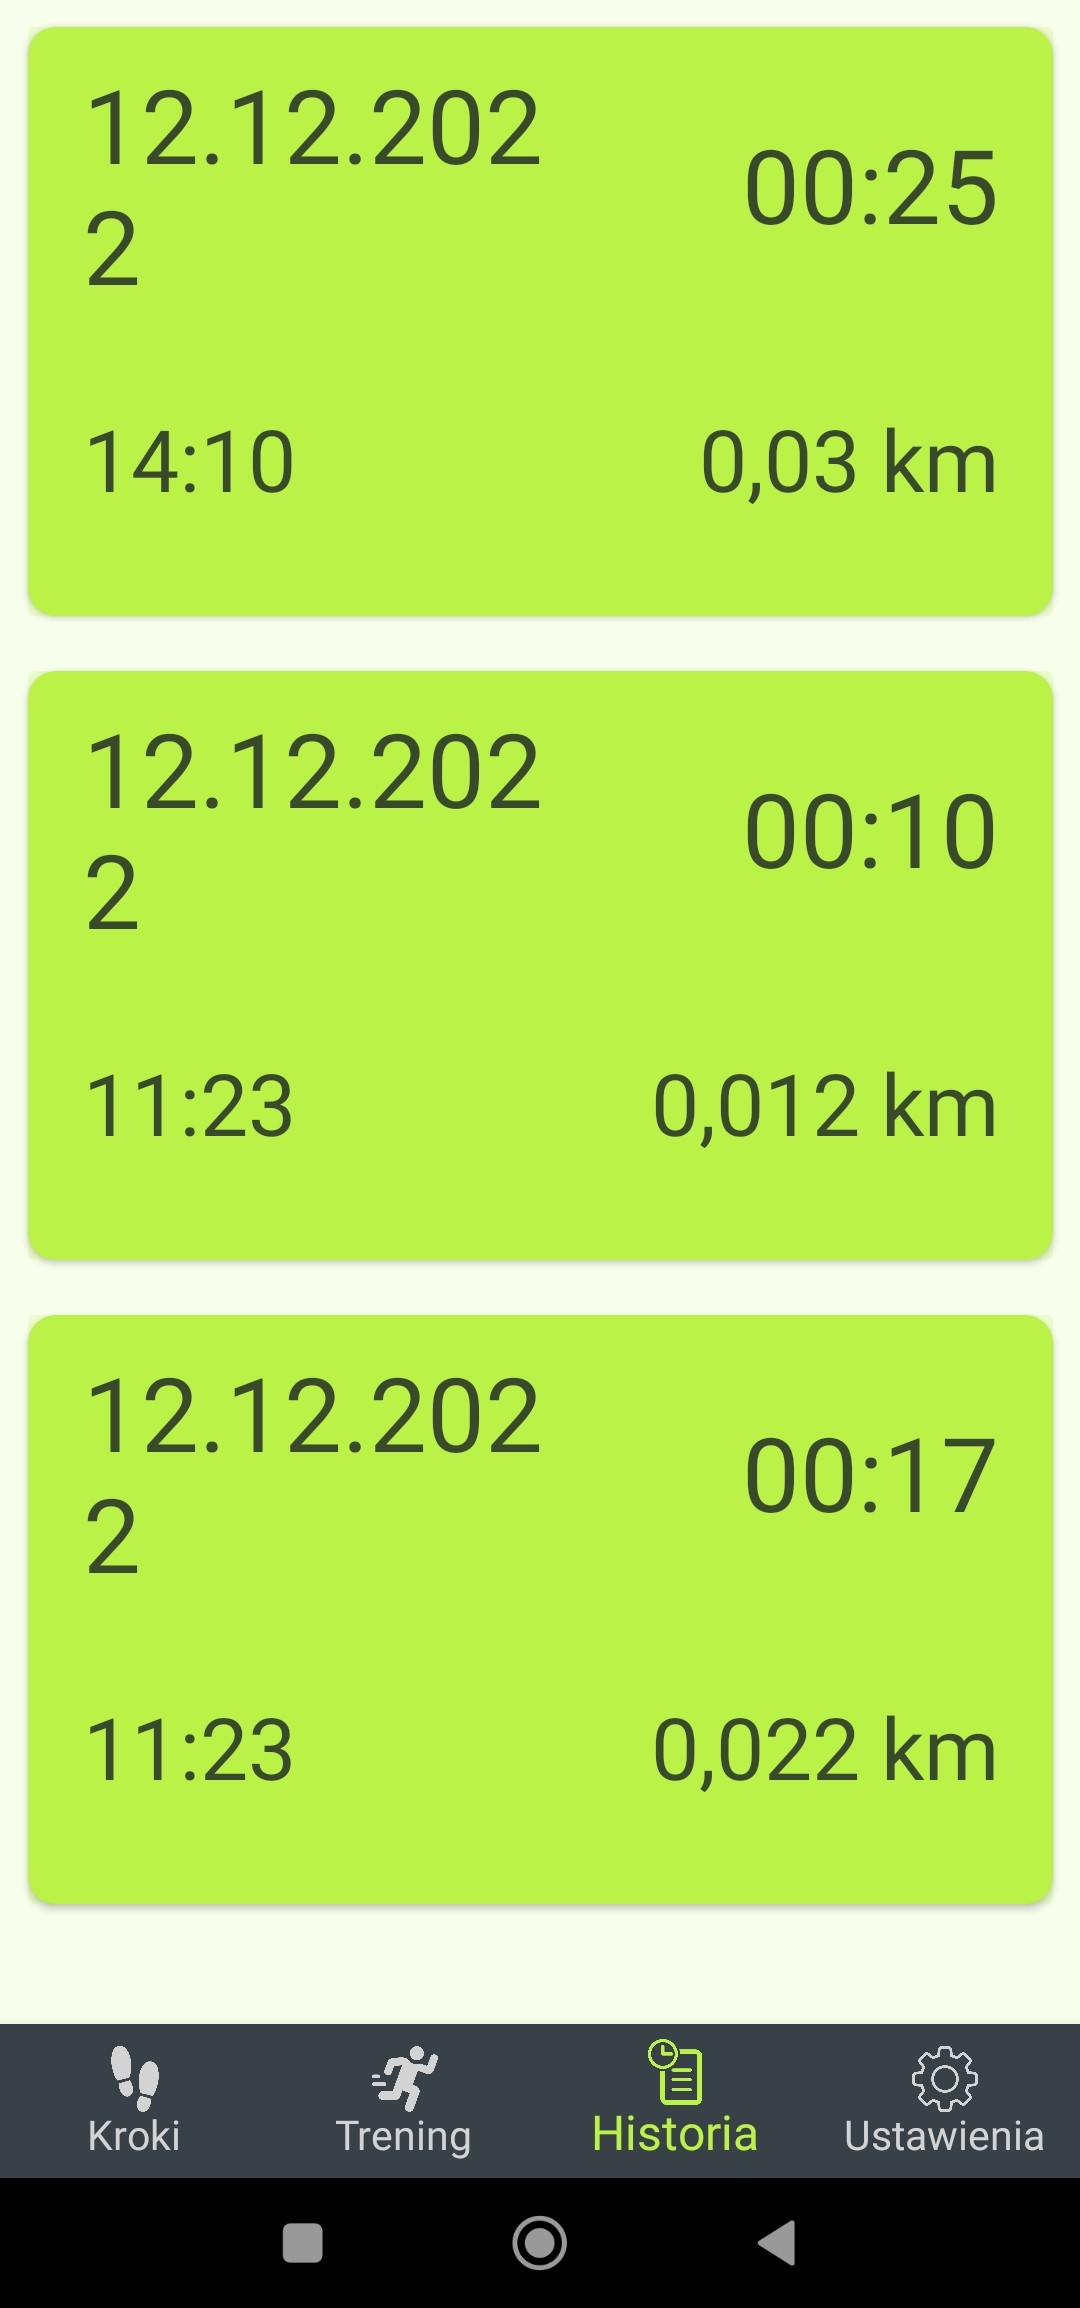
\includegraphics[width=.2\linewidth]{rys/historia2.jpg}
	\caption{Layout historii treningów}
	\label{rys:rysunek001d}
\end{figure}

Wykorzystana w nim zostaje odpowiednia funkcja otwierająca widok statystyk i podsumowania.

\subsubsection{Zakładka Ustawienia} %3.2.4

\hspace{0.60cm}W zakładce Ustawienia rys. \ref{rys:rysunek001e} (s. \pageref{rys:rysunek001e}) użytkownik ma możliwość konfiguracji własnego konta użytkownika, swoich danych fizycznych oraz wieku, na podstawie których obliczane zostają statystyki traningu jak np. spalone kalorie. 

\begin{figure}[!htb]
	\centering
	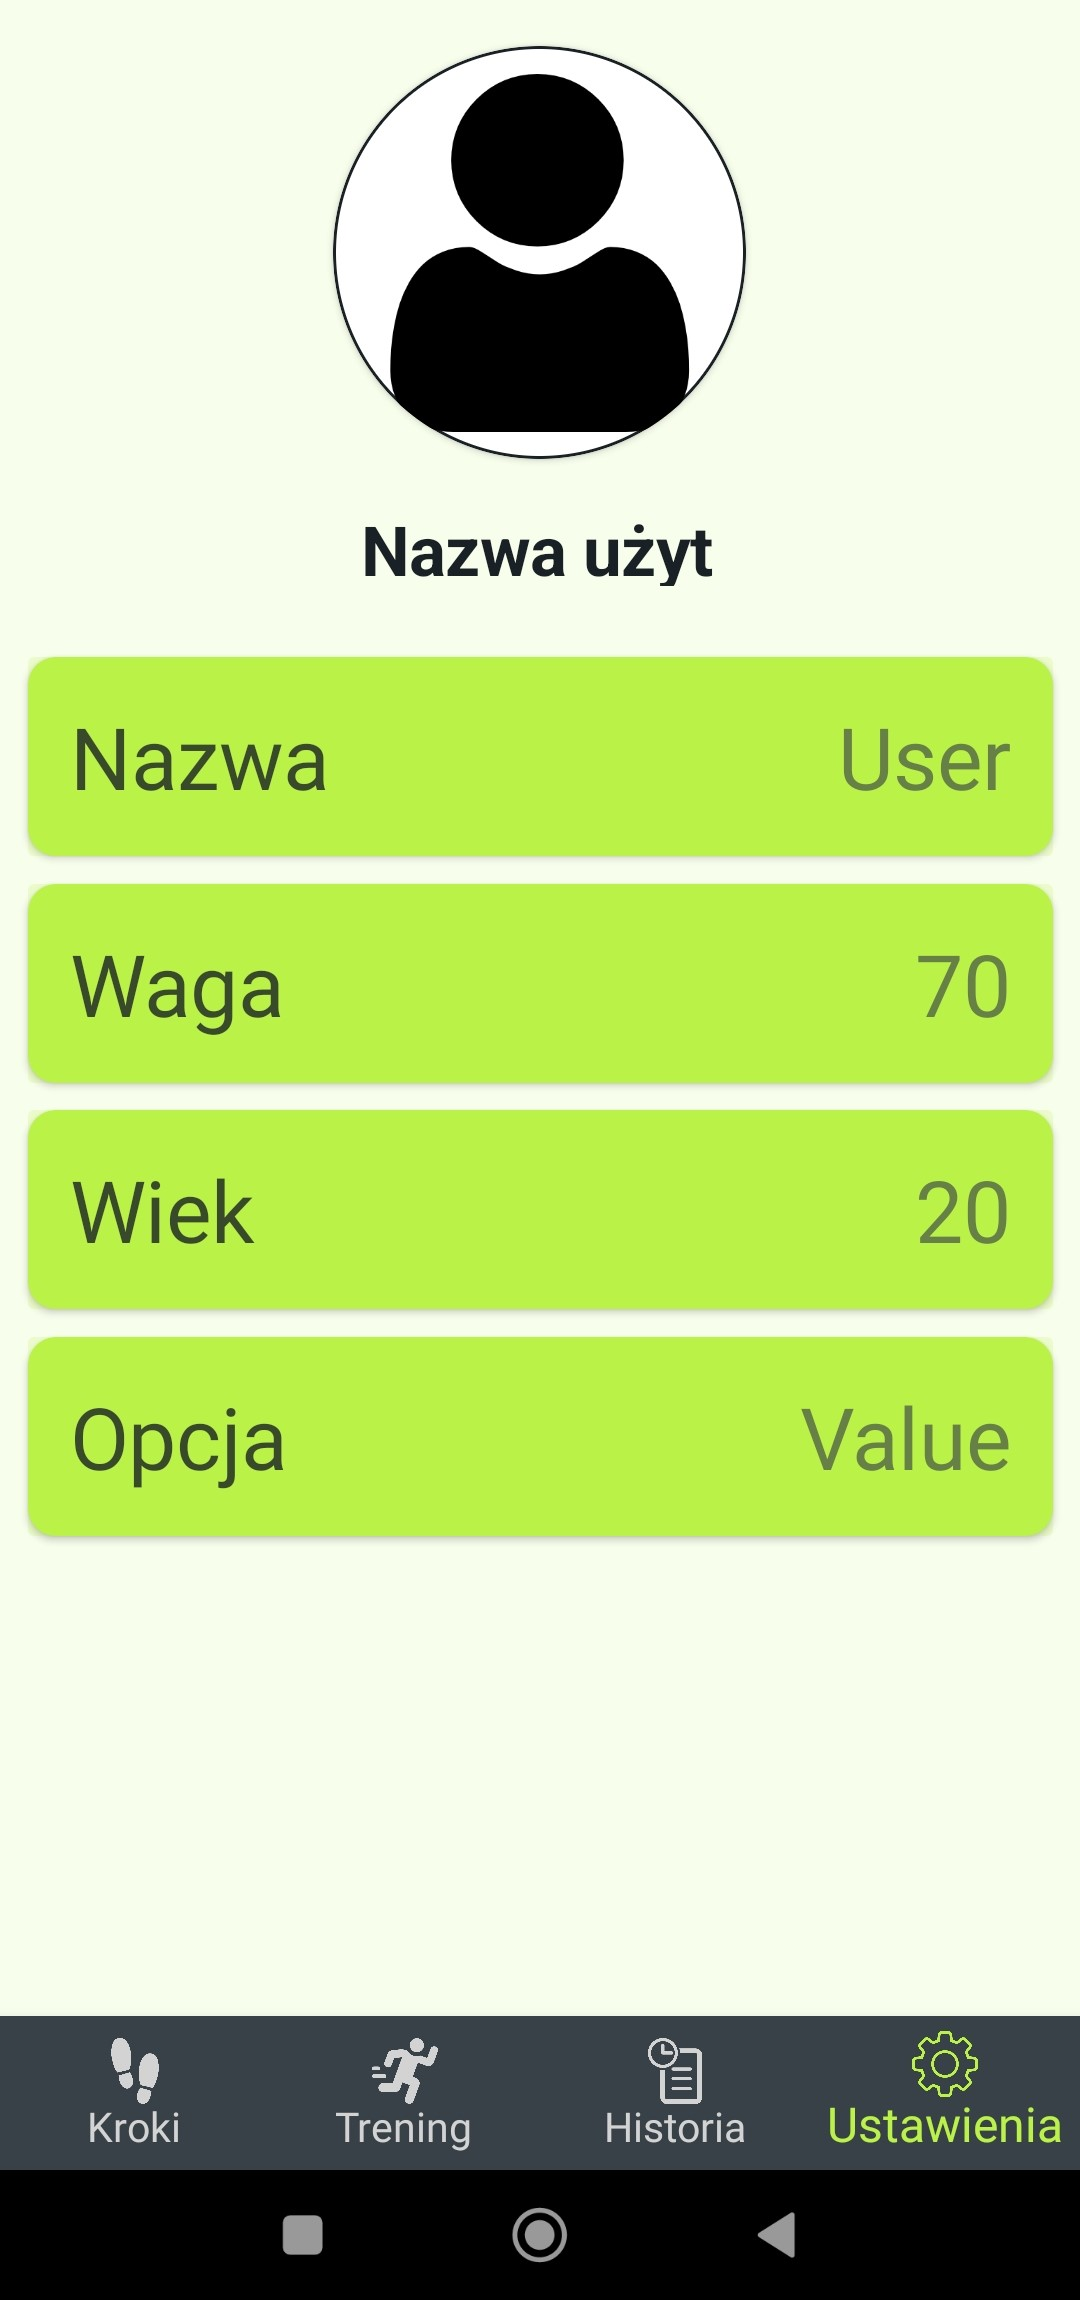
\includegraphics[width=.2\linewidth]{rys/ustawienia2.jpg}
	\caption{Layout ustawień i opcji}
	\label{rys:rysunek001e}
\end{figure}